		\subsection{Wstęp}
			\par Wykorzystanie systemu zarządzania i sklepu internetowego zapewnia ciągłość i bezpieczeństwo obiegu informacji. Wprowadza także sformalizowany sposób organizacji i zarządzania przedsiębiorstwem. Formalizacja ta zachodzi na polu organizacji procesów zamówienia i reklamacji. Systemowe podejście do tych procesów pozwala na śledzenie kondycji i planowanie działań przedsiębiorstwa.
			
		\subsection{Proces zamówienia}  
			\par Aby zorganizować proces zamówienia należy zachować dotyczące go dane celem późniejszego ich przetwarzania i kontroli jakości produktu. Podstawowymi danymi do zapamiętania będzie tu data wpłynięcia zamówienia, oraz data jego realizacji. Proces zamówienia składa się z dwóch pod procesów. Są nimi proces produkcji i logistyki.
			
			\par Dając klientowi możliwość wyboru opcji wykończenia danego produktu musimy zapisać wybrane przez niego opcje celem przekazania jednoznacznego zlecenia produkcji, możliwości kontroli poprodukcyjnej, oraz prawidłowego zabezpieczenia wysyłki. Dane te należy przekazać również na adres e-mail klienta. Negatywne zdarzenia, na jakie należy być przygotowanym to roszczenia klienta o niezgodność towaru, uszkodzenie w transporcie, kontrola skarbowa. Organizacja procesu sprzedaży w opisany sposób eliminuje konieczność posiadania magazynu. Zamówiony towar wyprodukowany wedle specyfikacji klienta zostaje do niego dostarczony z pominięciem magazynowania.
			
			\subsubsection{Produkcja}
				Organizacja produkcji. Dane do zabezpieczenia:
				\begin{itemize}
					\item Opcje wybrane przez klienta 
					\item Zlecenie produkcji wraz z terminami
					\item Zdjęcia po produkcyjne przed i po pakowaniu
				\end{itemize}
				
			\subsubsection{Transport}
				Organizacja transportu. Dane do zabezpieczenia:
				\begin{itemize}
					\item Sposób i terminy dostawy
					\item Dokumenty SAD w przypadku eksportu
				\end{itemize}
			
			\subsubsection{Przebieg procesu}
				\par Przebieg procesu zamówienia przestawia poniższy schemat blokowy. Zostały na nim uwzględnione czynności, jakie należy wykonać w odpowiedniej kolejności wraz z dokumentami, jakie należy wystawić i ich oczekiwać celem prawidłowego wykonania procesu zamówienia oraz uniknięcia konsekwencji prawnych.
			
				\begin{figure}[H]
					\centering
					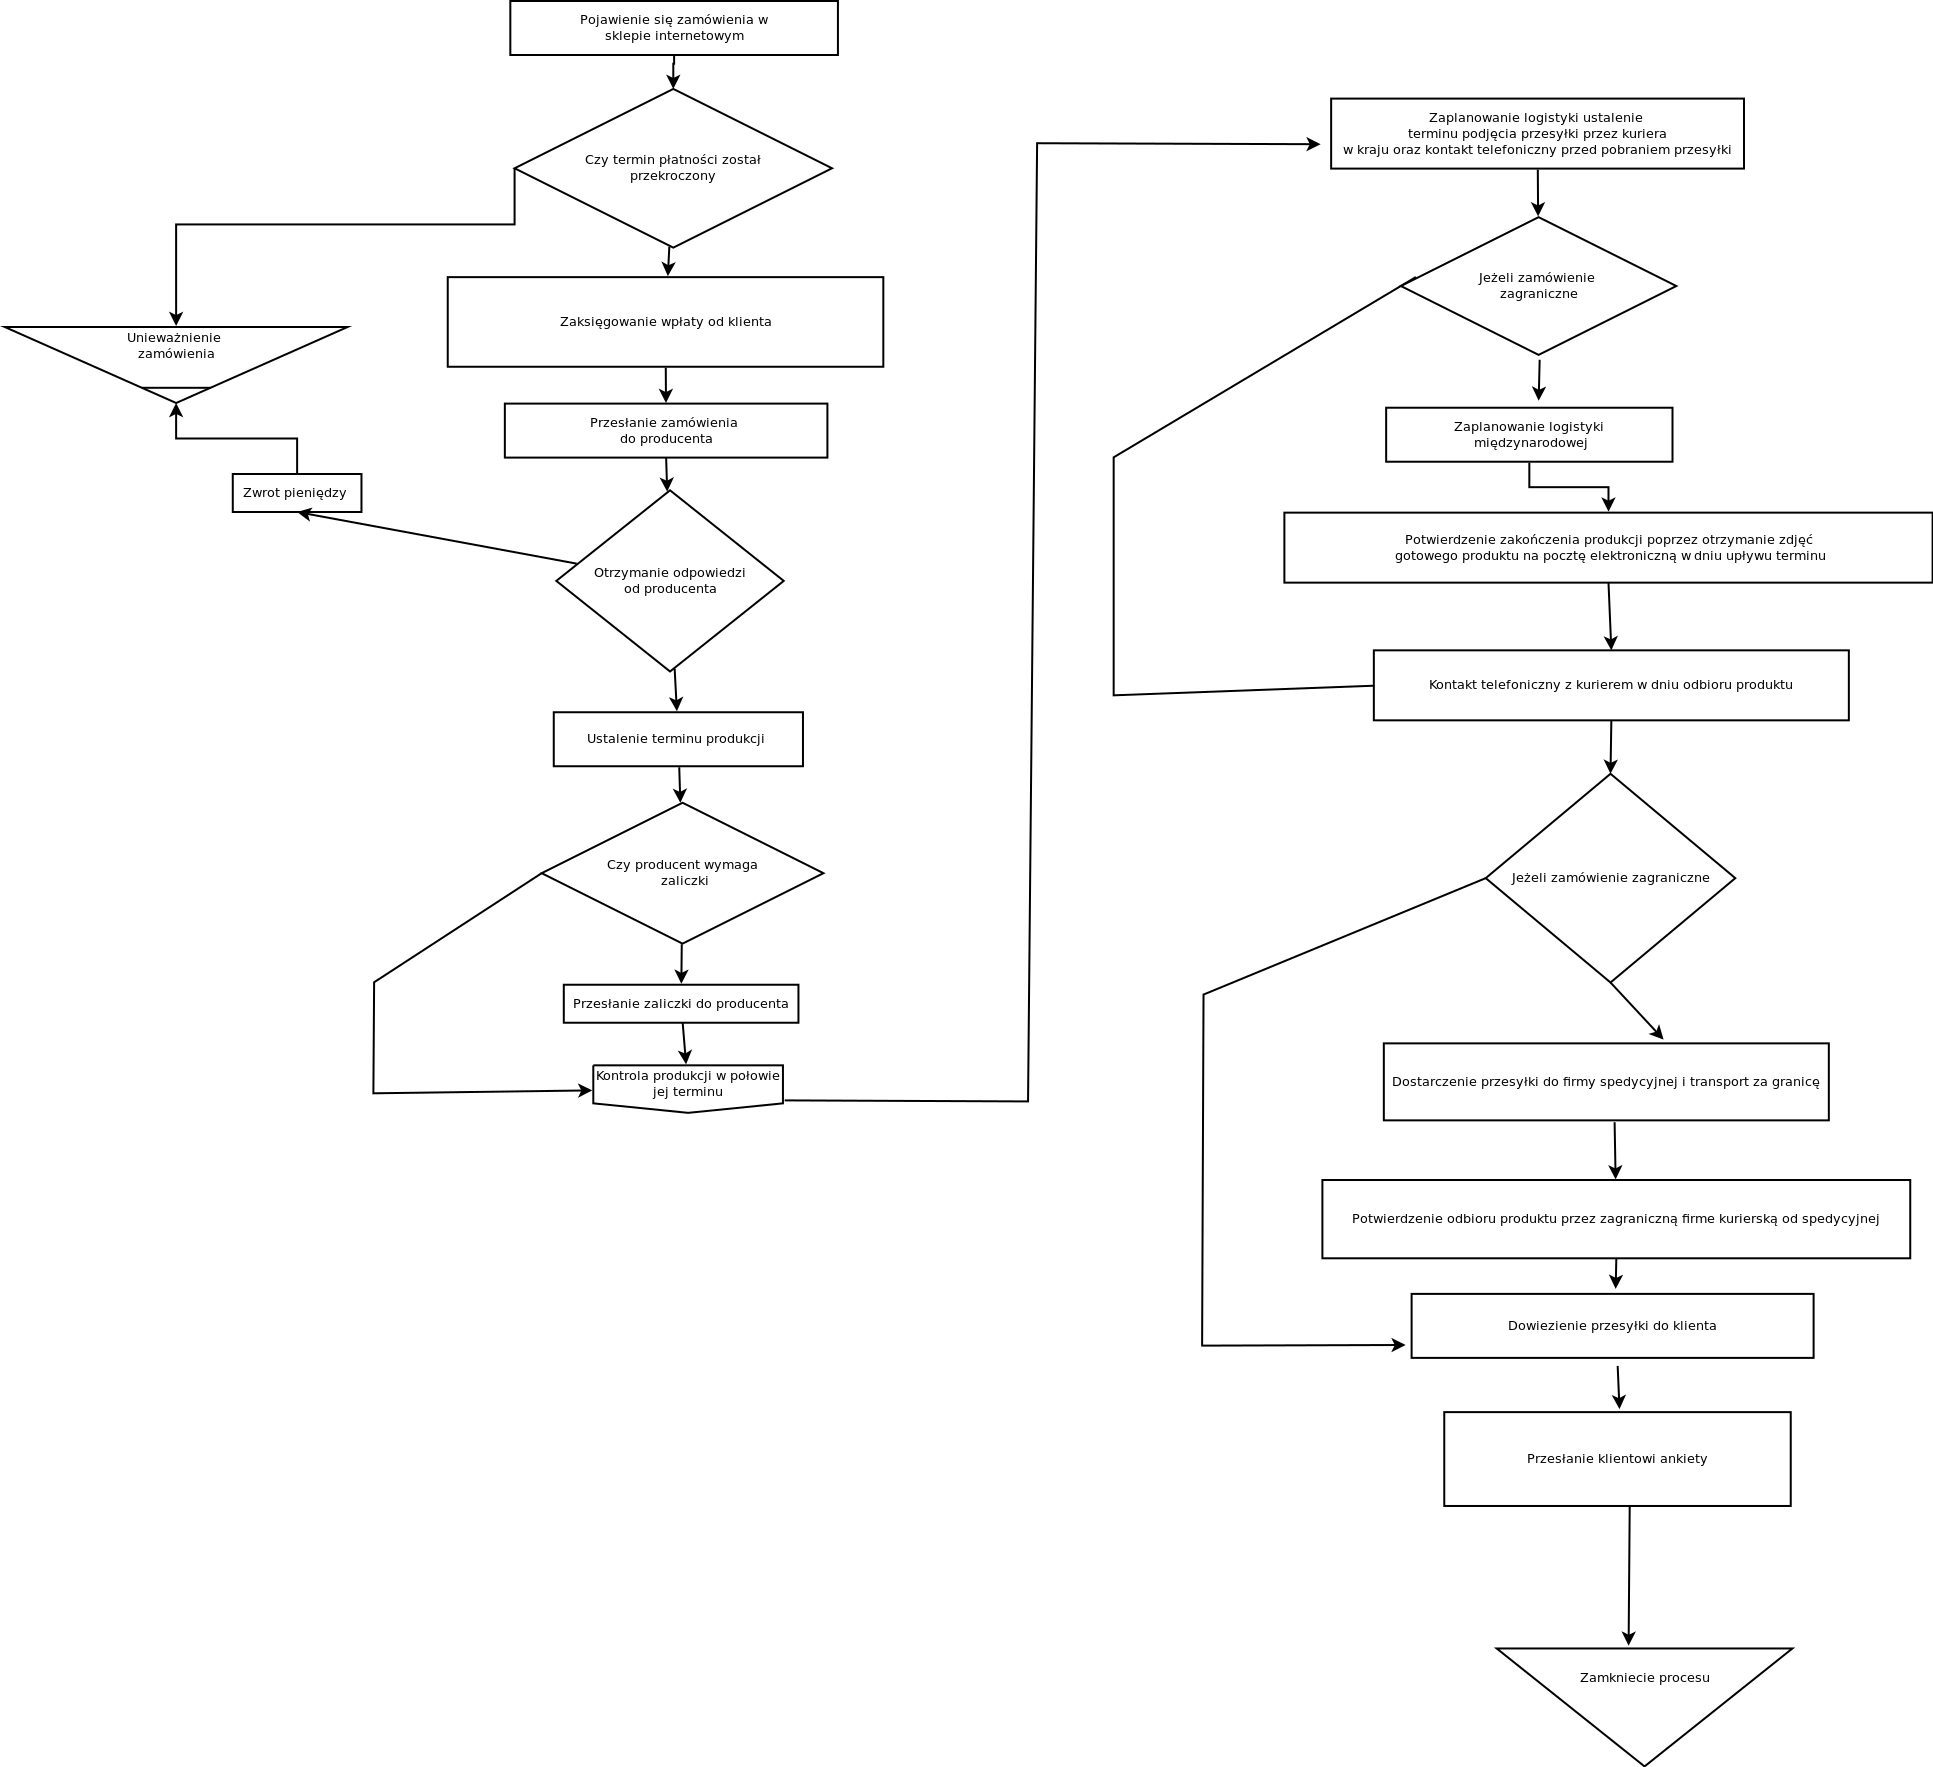
\includegraphics[scale=0.25]{zamowienie}
					\caption{Schemat procesu zamówienia}
				\end{figure}
			
		\subsection{Proces reklamacji}
			\par W tym procesie należy zabezpieczyć dane dotyczące zgłoszenia reklamacji, w skład których muszą wchodzić zdjęcia przedmiotu przesłane przez klienta w zgłoszeniu reklamacji. Na ich podstawie należy podjąć decyzję o uznaniu reklamacji lub odmowie. W wypadku uznania reklamacji i sprzedaży zagranicznej trzeba podjąć odpowiednią procedurę naprawy w kraju docelowym lub wysyłki nowego towaru z Polski i utylizacji uszkodzonego. W wypadku sprzedaży krajowej można zwrócić produkt do producenta celem usunięcia wad.
			
			
			\begin{figure}[H]
				\centering
				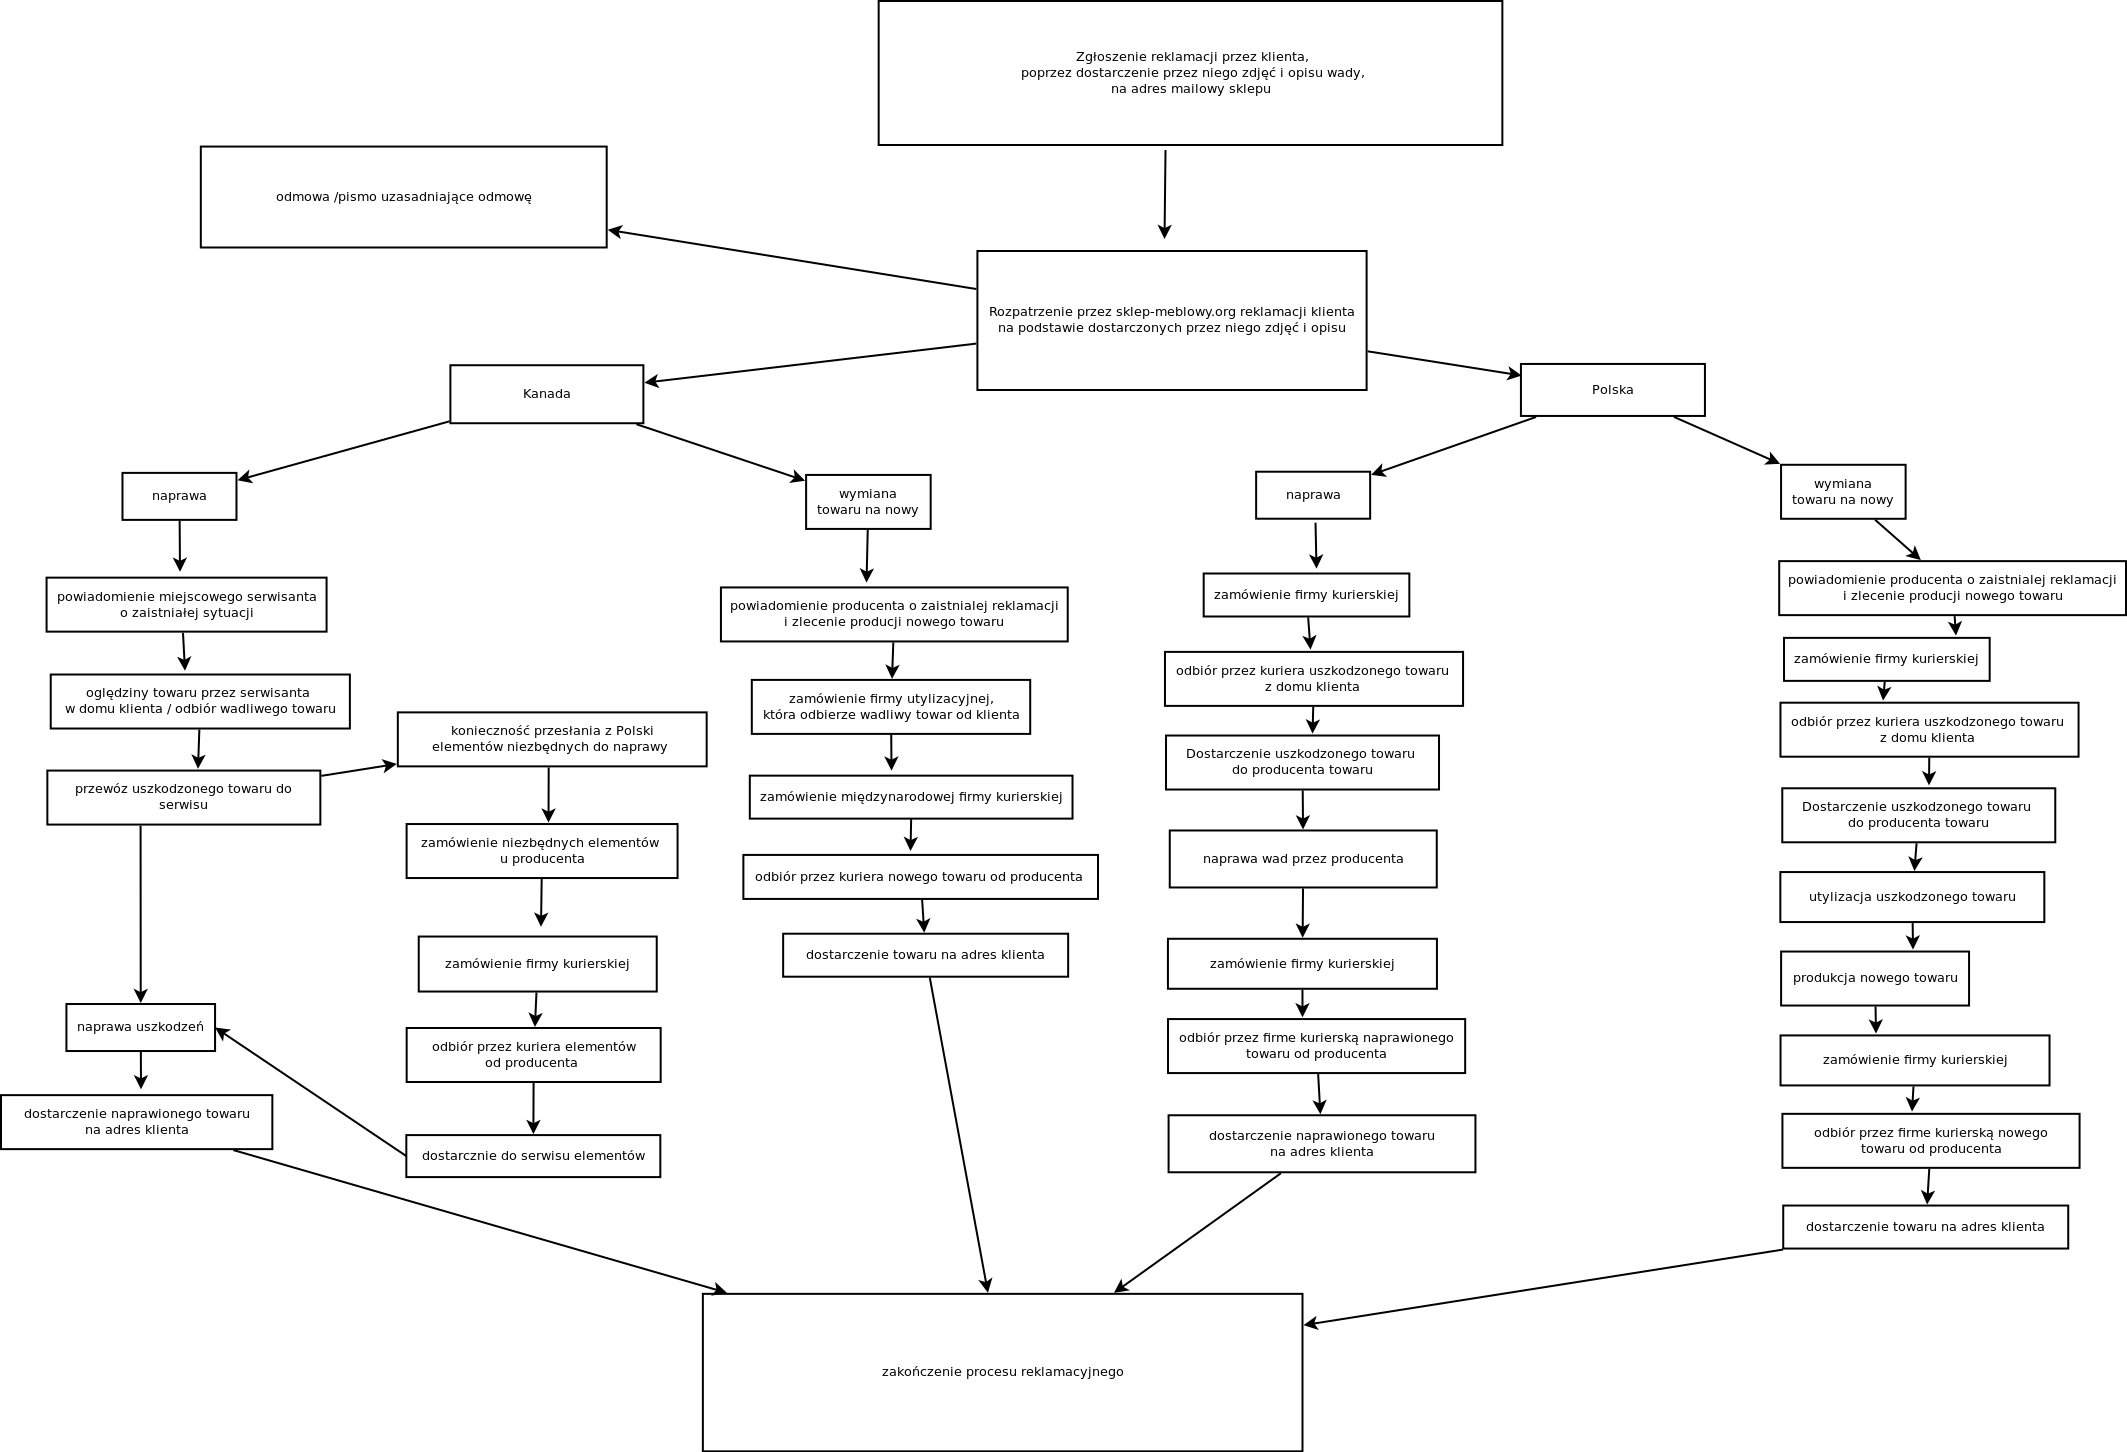
\includegraphics[scale=0.25]{reklamacja}
				\caption{Schemat procesu reklamacji}
			\end{figure}
			
